\documentclass[letterpaper,11pt]{article}

\usepackage{latexsym}
\usepackage[empty]{fullpage}
\usepackage{titlesec}
\usepackage{marvosym}
\usepackage[usenames,dvipsnames]{color}
\usepackage{verbatim}
\usepackage{enumitem}
\usepackage[hidelinks]{hyperref}
\usepackage{fancyhdr}
\usepackage[english]{babel}
\usepackage{tabularx}
\usepackage{fontawesome5}
\usepackage{multicol}
\setlength{\multicolsep}{-3.0pt}
\setlength{\columnsep}{-1pt}
\input{glyphtounicode}

%new packages

\usepackage{fontenc}
\usepackage{amsmath}
\usepackage{amssymb}
\usepackage{graphicx}



%----------FONT OPTIONS----------

\pagestyle{fancy}
\fancyhf{} % clear all header and footer fields
\fancyfoot{}
\renewcommand{\headrulewidth}{0pt}
\renewcommand{\footrulewidth}{0pt}

% Adjust margins
\addtolength{\oddsidemargin}{-0.6in}
\addtolength{\evensidemargin}{-0.5in}
\addtolength{\textwidth}{1.19in}
\addtolength{\topmargin}{-.7in}
\addtolength{\textheight}{1.4in}

\urlstyle{same}

\raggedbottom
\raggedright
\setlength{\tabcolsep}{0in}

% Sections formatting
\titleformat{\section}{
  \vspace{-4pt}\scshape\raggedright\large\bfseries
}{}{0em}{}[\color{black}\titlerule \vspace{-5pt}]



% Ensure that generate pdf is machine readable/ATS parsable
\pdfgentounicode=1

%-------------------------
% Custom commands
\newcommand{\resumeItem}[1]{
  \item\small{
    {#1 \vspace{-2pt}}
  }
}

\newcommand{\classesList}[4]{
    \item\small{
        {#1 #2 #3 #4 \vspace{-2pt}}
  }
}

\newcommand{\resumeSubheading}[4]{
  \vspace{-2pt}\item
    \begin{tabular*}{1.0\textwidth}[t]{l@{\extracolsep{\fill}}r}
      \textbf{#1} & \textbf{\small #2} \\
      \textit{\small#3} & \textit{\small #4} \\
    \end{tabular*}\vspace{-7pt}
}

\newcommand{\resumeSubSubheading}[2]{
    \item
    \begin{tabular*}{0.97\textwidth}{l@{\extracolsep{\fill}}r}
      \textit{\small#1} & \textit{\small #2} \\
    \end{tabular*}\vspace{-7pt}
}

\newcommand{\resumeProjectHeading}[2]{
    \item
    \begin{tabular*}{1.001\textwidth}{l@{\extracolsep{\fill}}r}
      \small#1 & \textbf{\small #2}\\
    \end{tabular*}\vspace{-7pt}
}


\newcommand{\resumeSubItem}[1]{\resumeItem{#1}\vspace{-4pt}}

\renewcommand\labelitemi{$\vcenter{\hbox{\tiny$\bullet$}}$}
\renewcommand\labelitemii{$\vcenter{\hbox{\tiny$\bullet$}}$}

\newcommand{\resumeSubHeadingListStart}{\begin{itemize}[leftmargin=0.0in, label={}]}
\newcommand{\resumeSubHeadingListEnd}{\end{itemize}}
\newcommand{\resumeItemListStart}{\begin{itemize}}
\newcommand{\resumeItemListEnd}{\end{itemize}\vspace{-5pt}}

\begin{document}
\fontfamily{cmr}\selectfont
\begin{center}
\parbox{3.0cm}{%
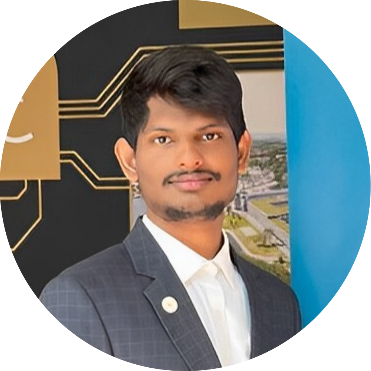
\includegraphics[width=2.7cm,clip]{images/resume_pic_m.png}}
}
\parbox{\dimexpr\linewidth-3.8cm\relax}{
\vspace{-20pt}
\begin{tabularx}{\linewidth}{L r} \\
    {\Huge \scshape  Venkata Sai Yakkshit Reddy Asodi}~
    \href{https://www.cedzlabs.com/yakkshit}{\vspace{1pt}}\\
      Sweden. \\ \vspace{1pt}
     \small \raisebox{-0.1\height}\faPhone\ +46 0793550685 ~ \href{mailto:saiyakkshit2001@gmail.com}{\raisebox{-0.2\height}\faEnvelope\  {saiyakkshit2001@gmail.com}} ~ 
    \href{https://linkedin.com/in/yakkshit/}{\raisebox{-0.2\height}\faLinkedin\ {yakkshit}}  ~
    \href{https://yakkshit.com/}{\raisebox{-0.2\height}\faGlobe\ {yakkshit.com}}  ~
    \href{https://github.com/yakkshit}{\raisebox{-0.2\height}\faGithub{ yakkshit}}
    \vspace{-8pt}
\end{tabularx}
}
\end{center}

\vspace{-23pt}
%-----------SUMMARY-----------
\section{Summary \faLink}
Frontend Developer and UI/UX specialist with a proven track record of building intuitive, data-driven web applications. Experienced in crafting user-centered interfaces from scratch and implementing complex data visualizations. Passionate about creating impactful solutions that bridge the gap between complex data and user-friendly experiences. Seeking to leverage my expertise in React and visualization libraries to help transform power grid data into meaningful insights at Endre Tech.

%-----------TECHNICAL SKILLS-----------
\section{\href{https://www.linkedin.com/in/yakkshit/details/skills/}{Technical Skills} \faLink}
\begin{itemize}[leftmargin=0.15in, label={}]
\small{\item{
\textbf{Frontend - }{React, TypeScript, JavaScript (ES6+), HTML5, CSS3, Tailwind, Apache ECharts} \\
\textbf{Design - }{Figma, UI/UX Design, Data Visualization, Responsive Design} \\
\textbf{Backend - }{RESTful APIs, Python, FastAPI} \\
\textbf{Tools - }{Git, GitHub, Zustand, Postman}\\
}}
\end{itemize}
\vspace{-10pt}

%-----------EXPERIENCE-----------
\section{Experience \faLinkedin}

\resumeSubHeadingListStart

\resumeSubheading
{\large Circleup AG \faBuilding}{December 2023 -- July 2024}
{Lead Frontend Engineer \& UI/UX Designer}{\faMapMarker \hspace{0.1cm} Zurich, Switzerland}\\
\vspace{10pt}
\textbf{Responsibilities:}
\resumeItemListStart
\vspace{-10pt}
\resumeItem{Led end-to-end UI/UX design and development, creating intuitive interfaces for complex data visualization dashboards. Implemented responsive design patterns and established a comprehensive design system.}
\resumeItem{Developed reusable React components and integrated various data visualization libraries to present complex analytics in an accessible format. Improved dashboard performance by 40\% through optimization techniques.}
\resumeItemListEnd
\vspace{-3pt}
\textbf{Environment:}\emph{React, TypeScript, Tailwind, RESTful APIs, Data Visualization Libraries}

\resumeSubheading
{Cedzlabs \faBuilding}{March 2023 -- July 2024}
{Full Stack Developer \& UI Designer}{\faMapMarker \hspace{0.1cm} India}\\
\vspace{10pt}
\textbf{Responsibilities:}
\vspace{-10pt}
\resumeItemListStart
\resumeItem{Spearheaded the design and development of user-centered web applications, focusing on data visualization and analytics dashboards. Collaborated directly with clients to gather requirements and iterate on designs.}
\resumeItemListEnd
\vspace{-3pt}
\textbf{Environment:}\emph{React, FastAPI, Python, Figma, Data Visualization Tools}

\resumeItem{\textbf{\href{https://linkedin.com/in/yakkshit}{Checkout my other experiences by clicking here}}}
\vspace{-5pt}

%-----------PROJECTS-----------
\section{Projects \faGithub}
\vspace{-5pt}
\resumeSubHeadingListStart
\resumeProjectHeading
{\textbf{\href{https://github.com/yakkshit/power-grid-analytics}{Power Grid Analytics Dashboard}} $|$ \emph{React, TypeScript, Apache ECharts}}{January 2024}\\
\vspace{6pt}
\textbf{Description:}
\vspace{-5pt}
\resumeItemListStart
\resumeItem{Developed a comprehensive dashboard for visualizing power grid data using React and Apache ECharts. Implemented interactive features for real-time data monitoring, trend analysis, and forecasting visualization. Created an intuitive UI that makes complex grid data accessible to non-technical users.}
\resumeItemListEnd
\vspace{4pt}
\textbf{Tools:}\emph{React, TypeScript, Apache ECharts, Tailwind, Zustand}
\vspace{-10pt}

\resumeProjectHeading
{\href{https://yakkshit.com}{\textbf{Data Visualization Portfolio}} $|$ \emph{React, D3.js}}{January 2023}\\
\vspace{6pt}
\textbf{Description:}
\vspace{-5pt}
\resumeItemListStart
\resumeItem{Created an interactive portfolio showcasing various data visualization projects, featuring responsive design patterns and modern UI/UX principles. Implemented complex visualizations using D3.js and React, demonstrating expertise in making data accessible and engaging.}
\resumeItemListEnd
\vspace{4pt}
\textbf{Tools:}\emph{React, D3.js, Figma, Responsive Design}
\vspace{-12pt}

%-----------ACHIEVEMENTS---------------
\section{Achievements / Contributions}
\resumeSubHeadingListStart
\resumeItemListStart
\resumeItem{Led the development of a design system that reduced development time by 30\% and improved consistency across applications.}
\resumeItem{Created and maintained open-source React components for data visualization, garnering 500+ GitHub stars.}
\resumeItem{Conducted workshops on modern UI/UX practices and data visualization techniques for development teams.}
\resumeItemListEnd

\resumeSubHeadingListEnd
\textbf{Strengths:}\emph{UI/UX Design, Data Visualization, Problem-solving, User-centered Design} \\
\textbf{Languages:}\emph{Telugu - Native $|$ English - Fluent $|$ Hindi - Fluent $|$ German - Elementary $|$ Swedish - Elementary}

\vspace{10pt}
\end{document}